% Rešerše – ERPNext (vkládá se do kapitoly 01-reserse.tex)
\section{ERPNext}\label{sec:reserse-erpnext}

ERPNext je open-source podnikový systém postavený na frameworku Frappe v~jazyce Python. Základní údaje shrnuje tabulka~\ref{tab:reserse-erpnext}.

\begin{table}[H]
\centering
\small
\begin{tabular}{>{\raggedright\arraybackslash}p{0.24\linewidth}>{\raggedright\arraybackslash}p{0.70\linewidth}}
\hline
\textbf{Kritérium} & \textbf{Zjištění} \\
\hline
Název & ERPNext \\
Společnost & Frappe Technologies Pvt. Ltd. (Indie) a~komunita; první verze v~roce 2010 \cite{wiki-erpnext} \\
Typ aplikace & webová aplikace (Python, framework Frappe, databáze MariaDB) \cite{wiki-erpnext,erpnext-web} \\
Hostování & vlastní server zdarma, nebo cloud Frappe Cloud \cite{erpnext-cenik} \\
Licence & open-source, GNU GPL v3; žádné funkce nejsou zpoplatněny \cite{erpnext-github,erpnext-web} \\
Cena & software zdarma; Frappe Cloud se neplatí za uživatele, ale podle výkonu: sdílený hosting od 5~USD, vlastní server od 20~USD měsíčně \cite{erpnext-cenik} \\
Zkušební verze & 14 dní na Frappe Cloud \cite{erpnext-cenik} \\
\hline
\end{tabular}
\caption{Základní údaje o~řešení ERPNext}\label{tab:reserse-erpnext}
\end{table}

\subsection{Zkušenosti ze zkušební verze}

Průvodce prvním nastavením se zobrazil v~angličtině a~aplikace byla proto hodnocena v~anglickém prostředí. Projekt sice obsahuje komunitní český překlad rozhraní \cite{erpnext-github}, oficiální česká lokalizace (například podpora formátu ISDOC nebo českých daňových výkazů) však neexistuje \cite{frappe-forum-cz}.

Rozhraní působí minimalisticky a~přehledně: v~levé části je lišta s~ikonami modulů, jejichž název se zobrazí po najetí myší, a~vedle ní seznam podkategorií. Sekce \emph{Setup} nabízí velké množství možností, od správy uživatelů, organizace a~přístupových rolí po nastavení tiskových dokumentů, včetně úpravy hlavičky dokumentu v~jazyce HTML. Všechny volby jsou přehledné a~tlačítka pro uložení nebo přidání záznamu jasně viditelná, celkově však aplikace působí jako nástroj pro zkušeného administrátora, který si systém sám nastaví, nikoli pro běžného zaměstnance malé firmy. Bez zaškolení by úvodní nastavení zabralo několik hodin. Příjemně jednoduché je založení nového uživatele, kde stačí vyplnit e-mail a~jméno, s~možností zobrazit celý formulář. Panel upozornění je funkční (všechna upozornění nebo jen nadcházející události), ale zobrazuje se přes celou výšku stránky a~zakrývá obsah (obrázek~\ref{obr:erpnext-upozorneni}). Evidence zakázek je vedena prostřednictvím projektů, takže každá servisní zakázka by musela být založena jako samostatný projekt, což je pro servisní praxi zbytečná administrativní zátěž.

\begin{figure}[H]
\centering
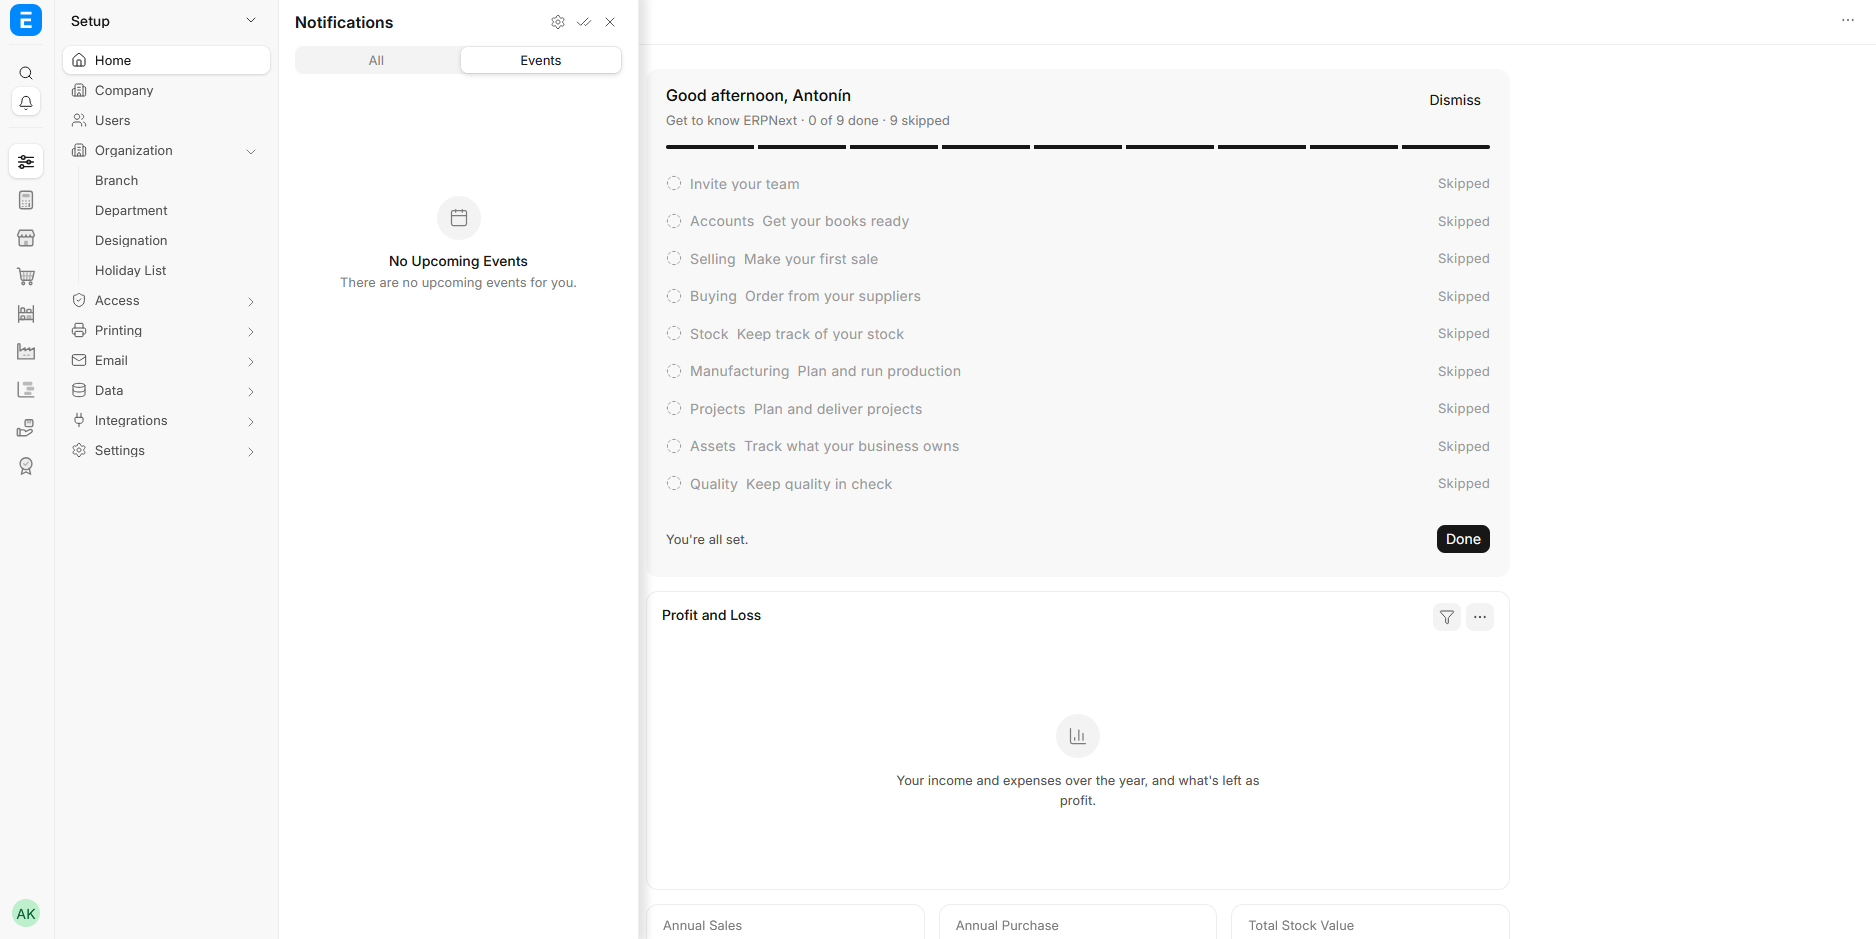
\includegraphics[width=\linewidth]{obrazky/reserse/erpnext_upozorneni.png}
\caption{Panel upozornění v~ERPNext zobrazený přes celou výšku stránky (zdroj: vlastní snímek obrazovky ze zkušební verze, pořízeno 3.~11.~2026)}\label{obr:erpnext-upozorneni}
\end{figure}

\subsection{Vhodnost pro malé firmy}

Cenově je ERPNext pro malou firmu velmi vhodný: software je zdarma a~cloudový provoz se neplatí za uživatele. Překážkou je však chybějící česká lokalizace, nedostatek implementačních partnerů v~České republice a~náročnost nastavení i~vlastního provozu, který vyžaduje znalost Linuxu, Pythonu a~databáze MariaDB. Pro malou servisní firmu bez technického zázemí je proto nasazení obtížné. Architekturou, tedy open-source webovou aplikací v~jazyce Python, je však ze všech srovnávaných řešení navrhované aplikaci nejblíže.
